\section{Experimental setup}
\label{sec:experimental_setup_}
Modern experimental physics use large circular collider in order to approach the center of mass energies necessary for the
specific resonances. In particular, the Large Electron-Positron Collider (\textbf{LEP}) whose data we are using was one
of the largest accelerator ever constructed with a circumference of 27 kilometres. Electron- and positron packets are brought
to energies from $\sqrt{s} = 88$ GeV up to $\sqrt{s} = 94$ GeV in order to examine the gauge bosons of the weak interaction. 
The Experiments \textbf{OPAL}, \textbf{DELPHI}, \textbf{ALEPH} and \textbf{L3} were conducted to measure the electron positron
collisions, but we will only look at \textbf{OPAL}. 
We will give a detailed description in the next
subsection below.


\subsection{\textbf{OPAL}: The Hunt for $Z^0$}
\label{sub:OPAL}
Its abbreviation stands for  "\textbf{O}mni \textbf{P}urpose \textbf{A}pparatus at \textbf{L}EP". The experiment started in
1989 and data was taken until the year 2000. The collaboration consisted of 200 physicists from 34 institutes.
The main ingredients of the experiment are the following: 
\begin{itemize}
    \item \emph{Tracking Detectors} 
    \item[Tracking Detectors]
\end{itemize}
\begin{figure}[htpb]
    \centering
    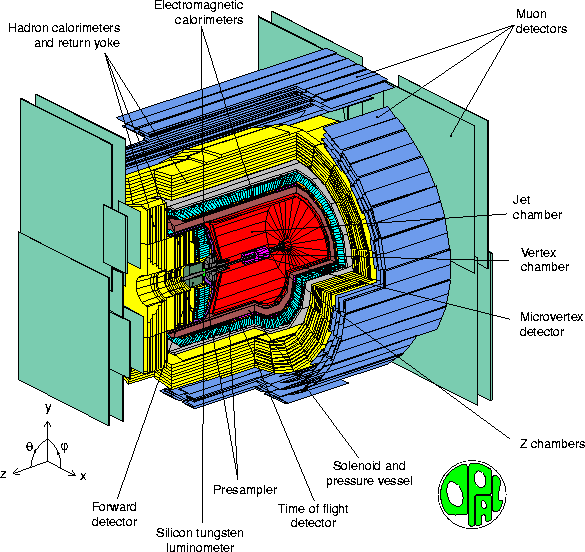
\includegraphics[width=1.0\linewidth]{figures/opal}
    \caption{The image shows a cut-away view of the \textbf{OPAL} detector\cite{CERN_OPAL}. The layered structure of the
    different chambers, which encase the central beam pipe can be distinguished clearly. 
    }
    \label{fig:opal1}
\end{figure}

\begin{figure}[htpb]
    \centering
    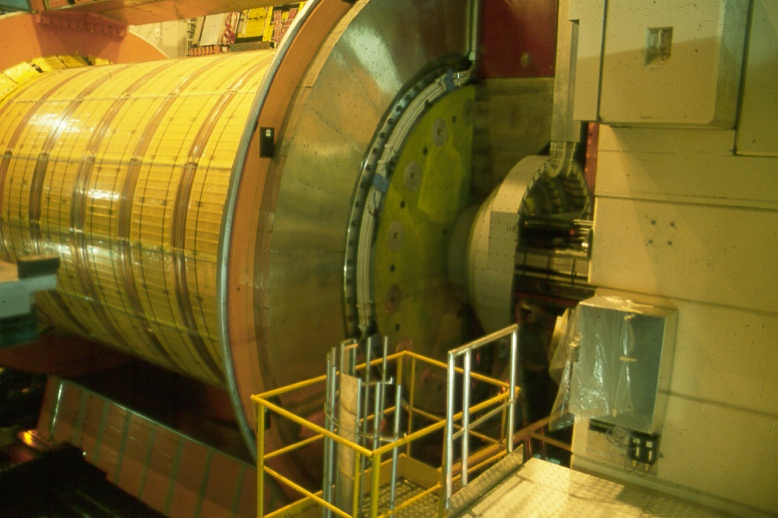
\includegraphics[width=1.0\linewidth]{figures/opal_photo}
    \caption{Photography of the early installation, spring 1988\cite{CERN_OPAL}. The experiments extents were
    $12m \times 12m \times 12m$ and was dismantled in 2001 due to to the construction of the LHC. To the right you can 
see outer structure of the detector, for more technical details refer to figure~\ref{fig:opal1}. }
    \label{fig:opal_photo}
\end{figure}
